\documentclass[conference]{IEEEtran}
\usepackage{cite}
\usepackage{amsmath,amssymb,amsfonts}
\usepackage{algorithmic}
\usepackage{graphicx}
\usepackage{textcomp}
\usepackage{hyperref}

\graphicspath{{figs/}}
\begin{document}

\title{Teaching Robots how to Interact with Humans}

\author{\IEEEauthorblockN{Emmanuel Senft}
\IEEEauthorblockA{\textit{Centre for Robotics and Neural Systems} \\
\textit{Plymouth University} \\
Plymouth (UK) \\
emmanuel.senft@plymouth.ac.uk\\
\url{http://www.tech.plym.ac.uk/SoCCE/CRNS/staff/esenft/}}
}

\maketitle

\begin{abstract}

To have meaningful social interaction with humans, robots have to be able to improve
    their behaviour over time by learning from humans. My research is
    focused on how a robot can learn how to interact with humans while
    interacting with someone and being supervised by a teacher.

\end{abstract}

\section{Introduction}

Social interactions are complex environments governed by a large number of
social norms and where any participants have a high number of expections on the
others.  As it seems impossible to provide directly a robot with all the
knowledge required to interact with humans, we argue that robots need to be able
to learn how to interact socially. Furthermore, as the context of interaction
and the partners can evolve over times, robots have to continuously update their
behaviour.  The problem of improving an action policy over time by interacting
in an environment is well represented by Reinforcement Learning. Powerful tools
exist to improve an agent behaviour as it is evolving in an environment. By
maximising a reward function rating behaviours of the agents, it can improve its
behaviour to behaviour over time. 

However classic method in Reinforcement Learning are relying on exploration,
often random to acquire information on the environment and generally requires
many iterations to converge to an appropriate action policy. When interacting
with humans in the real world, acquiring data can take a prohibitive time, and
the risk of exploration can be high: failing to satisfy expectations from human
partners can lead to the end of the interaction or annoy the partners. To tackle
this issue, we propose to make use of a human supervisor to guide the robot
behaviour, preventing it to make mistakes and demonstrating it a correct action
policy.

\section{Proposition}

\subsection{Supervised Autonomy}

Robots cannot have optimal behaviours, especially in the early stages of
learning. The idea behind Supervised Autonomy is to have a robot mostly
autonomous, but supervised by a human. Before executing an actions, the robot
proposes this action to a supervisor who is able to correct it before execution,
ensuring that only actions validated by a human are executed. 

This validation of action is combined with an automatic execution after a short
delay: for all correct actions, the supervisor does not have to act and can let
the robot being autonomous, only in cases where the proposed action is
incorrect, the supervisor has to step in.

\subsection{SPARC}

When the robot is interacting in a Supervised Autonomous fashion, it can also
use the human inputs to improve its behaviour over time. Combined with
algorithms from the Reinforcement Learning field or other direct mapping
inputs-action, this approach ensures that the behaviour of the robot is
constantly correct and the frequency of intervention from the supervisor
decreases as the robot learns.

Other methods using humans to teach a robot how to interact often use the human
only to label actions from the robot, to provide corrective behaviours once the
robot has made a mistake or have the robot request a demonstration from the
human when its confidence in the output of the learning algorithm is too low.
On the other hand, SPARC aims to give control over the robot's action to a
teacher to ensure a high performing action policy at every step of the
interaction.  Figure~\ref{fig:comparison} show an illustrative comparison
between SPARC and other learning methods. By giving control on \emph{every}
robot's action to the teacher, SPARC is the only method allowing the robot to
have an efficient behaviour even in early stages of the learning while reducing
the number of actions from the teacher over time.

\begin{figure}
    \centering
    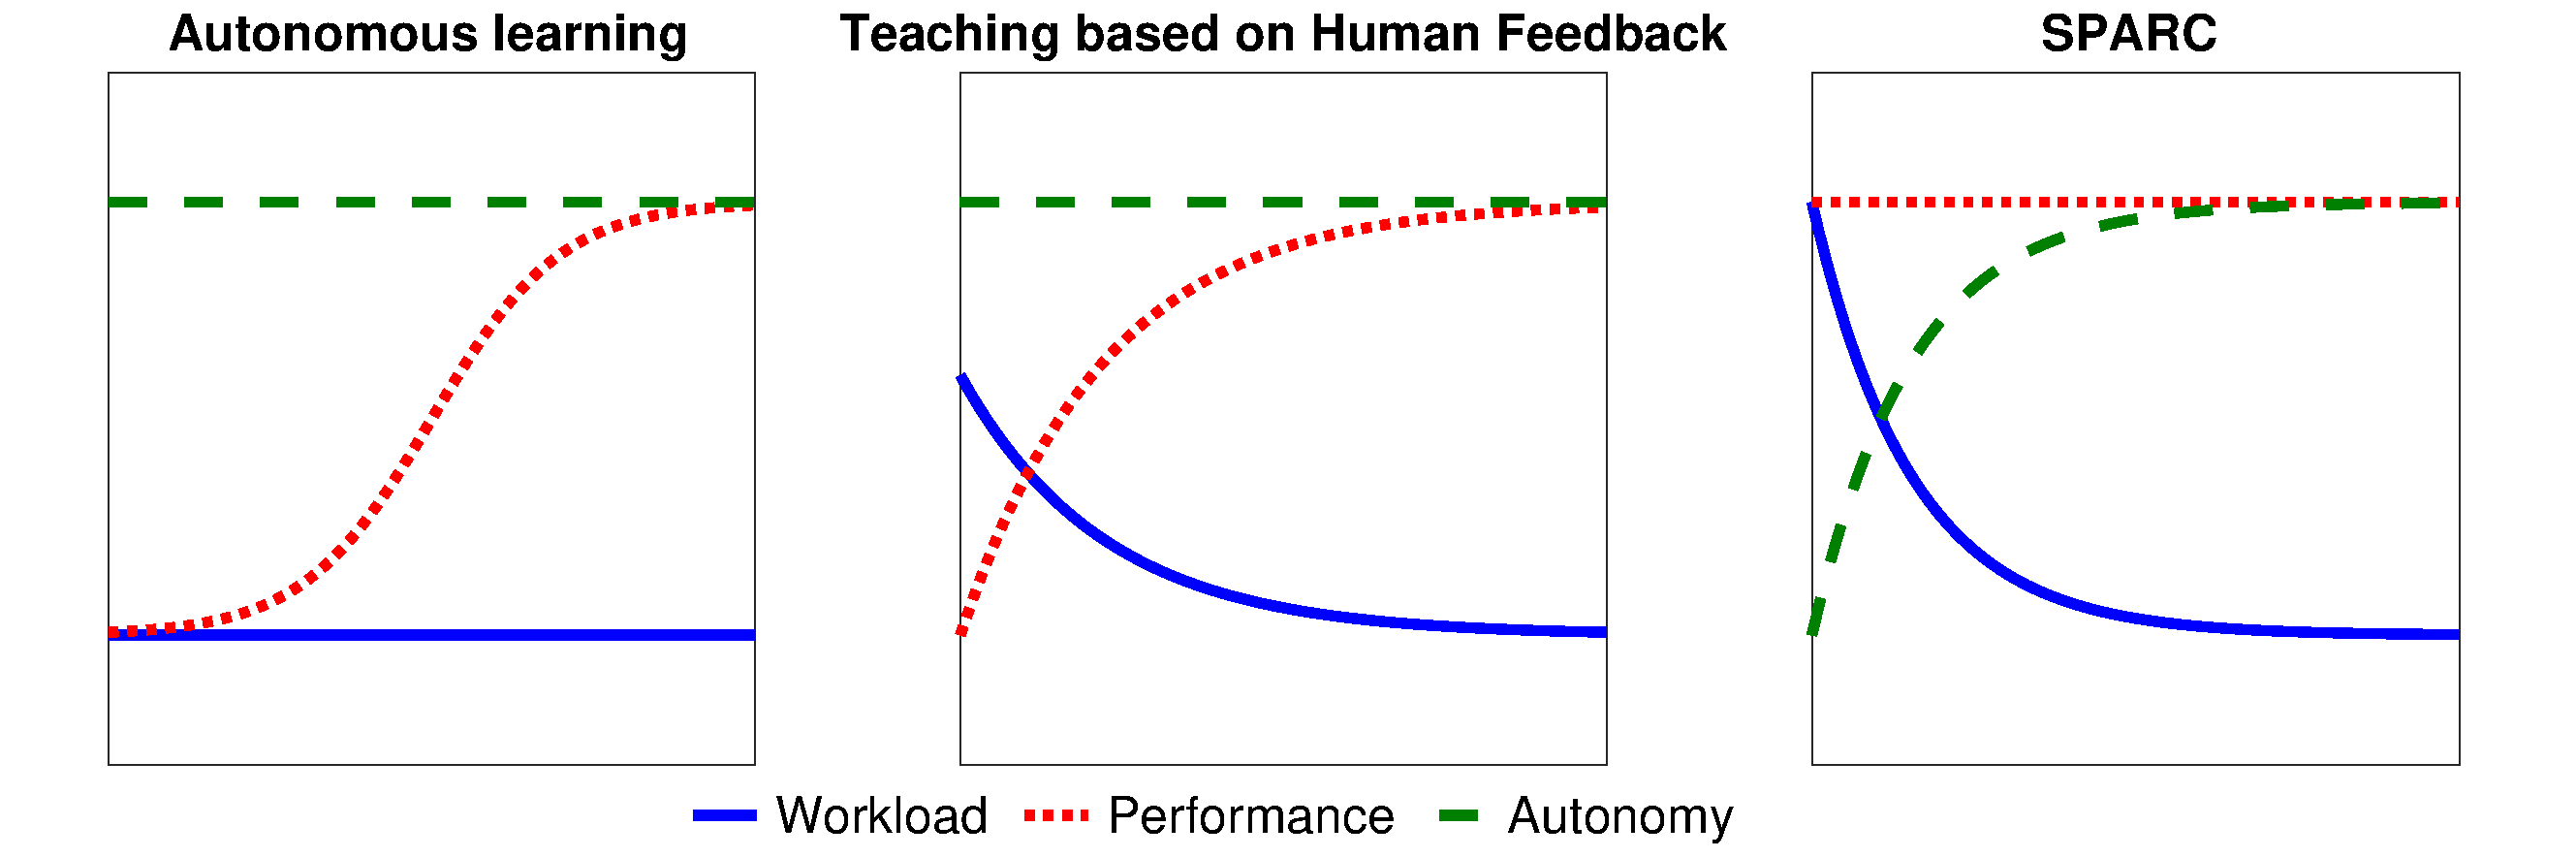
\includegraphics[width=0.9\linewidth]{motivation.pdf}
    \caption{Comparison of workload on human teacher, performance of the robot
    and autonomy for three frameworks of learning: autonomous learning, learning
    with human feedbacks and SPARC}
    \label{fig:comparison}
\end{figure}

\section{Experiments}

SPARC has been tested in two explorative studies and so far has demonstrated
promising results.

\subsection{Initial Eploration with Direct Mapping}

The first study \cite{senft2015sparc} involved 10 participants teaching a teacher robot how to provide
feedbacks to a learner in a classification task. For the sake of the study, the
learner was modeled by a second robot with a behaviour impacted by the teacher
robot. This study used a simple feedforward neural network to map state to
action. As shown in Figure~\ref{fig:ICSR}, compared to Wizard of Oz interaction
(the human has to select manually all the actions executed by the robot), SPARC
can achieve a similar performance while requiring a lower number of inputs.

\begin{figure}
    \centering
    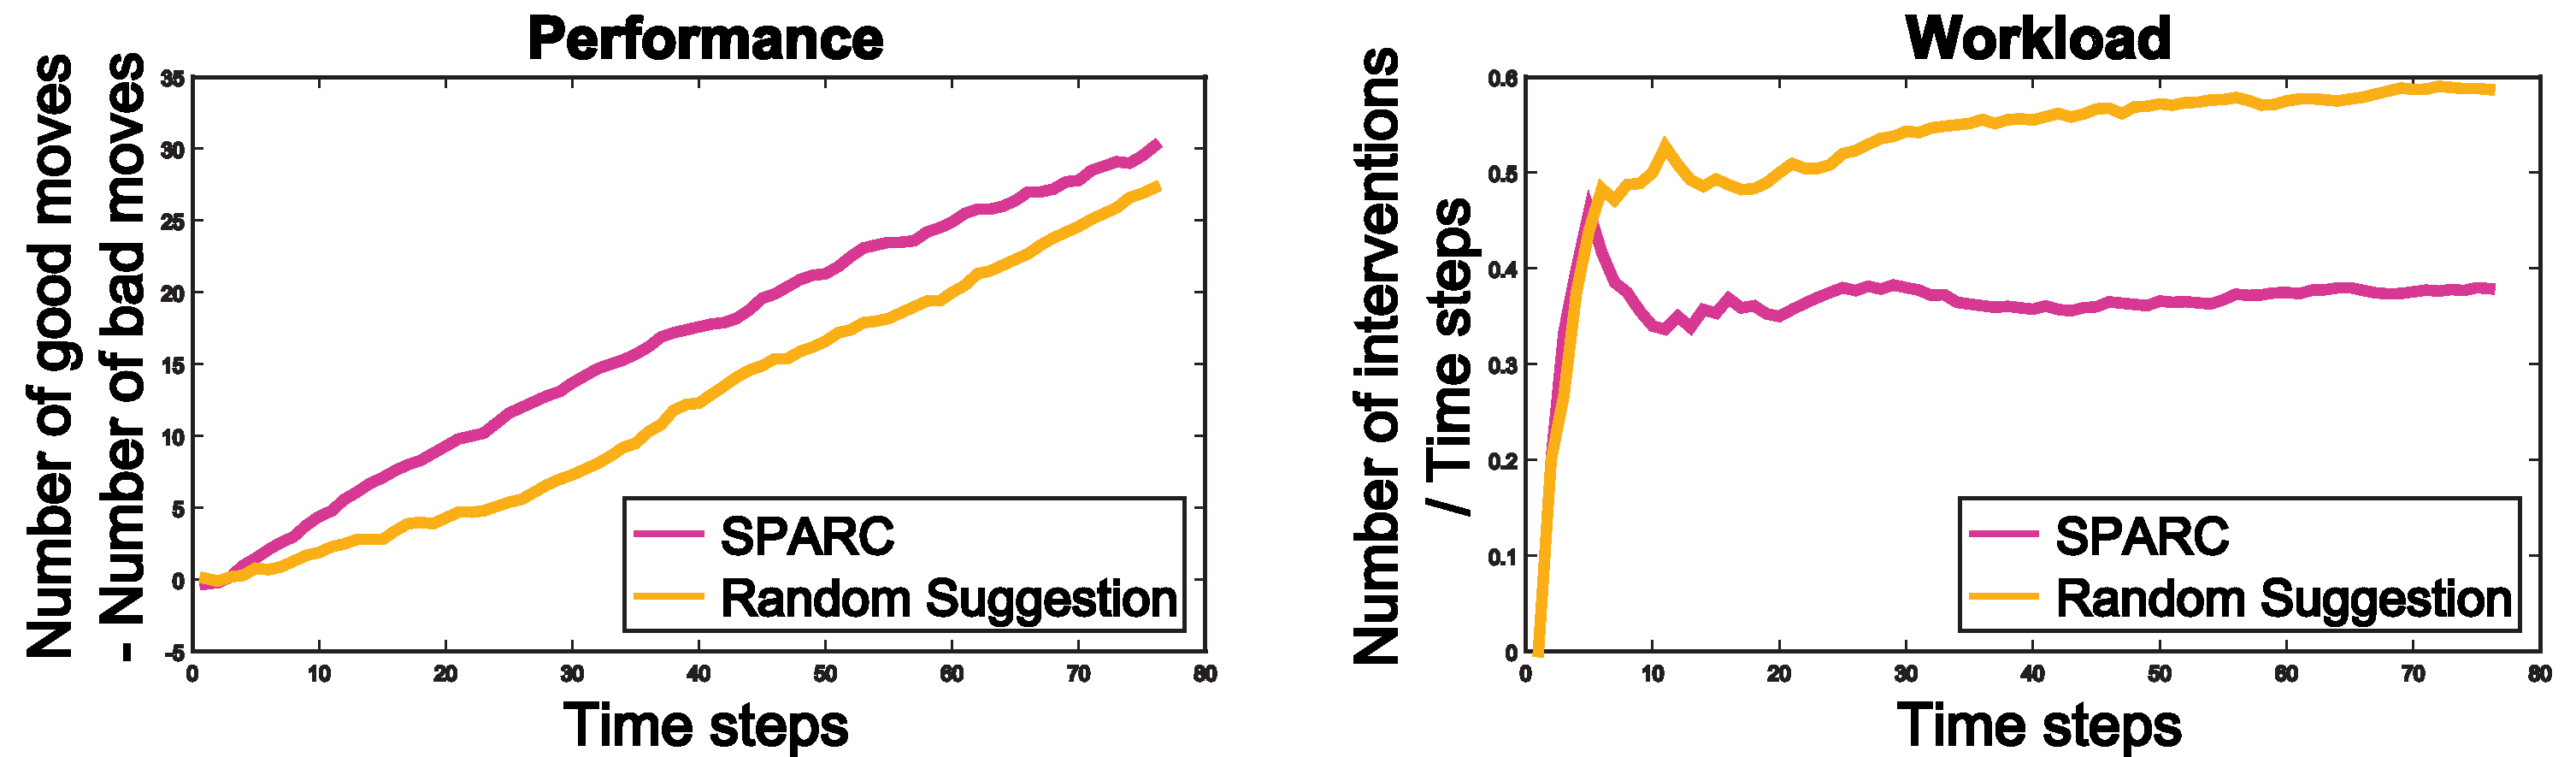
\includegraphics[width=0.9\linewidth]{ICSR.pdf}
    \caption{Comparison of workload on human teacher and performance of the robot
    for two control scenario: SPARC and a random suggestion equivalent to a
    Wizard of Oz control}
    \label{fig:ICSR}
\end{figure}


\subsection{Combining Supervised Autonomy with Reinforcement Learning}

The second study \cite{senft2017supervised} used Sophie's Kitchen, the
environment proposed by Thomaz and Breazeal in~\cite{thomaz2008teachable} to
explore how a human supervisor can teach a robot to complete a task in a
deterministic environment. The learning algorithm is from the Reinforcement
Learning field, the agent receives rewards and learns how to maximise the
rewards obtained to reach an efficient action policy and complete the task. This
study involved 40 participants teaching the robot how to complete the task in
two condition. In the Interactive Reinforcement Learning, the teacher can
provide feedbacks and provide guidance to the robot to execute some actions. In
the second condition, SPARC, the teacher is informed of which action the robot
is about to execute and can correct it before execution. With SPARC, the rewards
are implicit, each action executed by the robot is rewarded with $+1$ as it
received the approval from the teacher either explicitely (if selected) or
implicitely (if letting be executed). 

As shown in Figure~\ref{fig:film}, during the first interaction with an
algorithm, participants reached a higher performance with SPARC compared to IRL,
while requirering less inputs, less time and reaching less failure states.

\begin{figure}
    \centering
    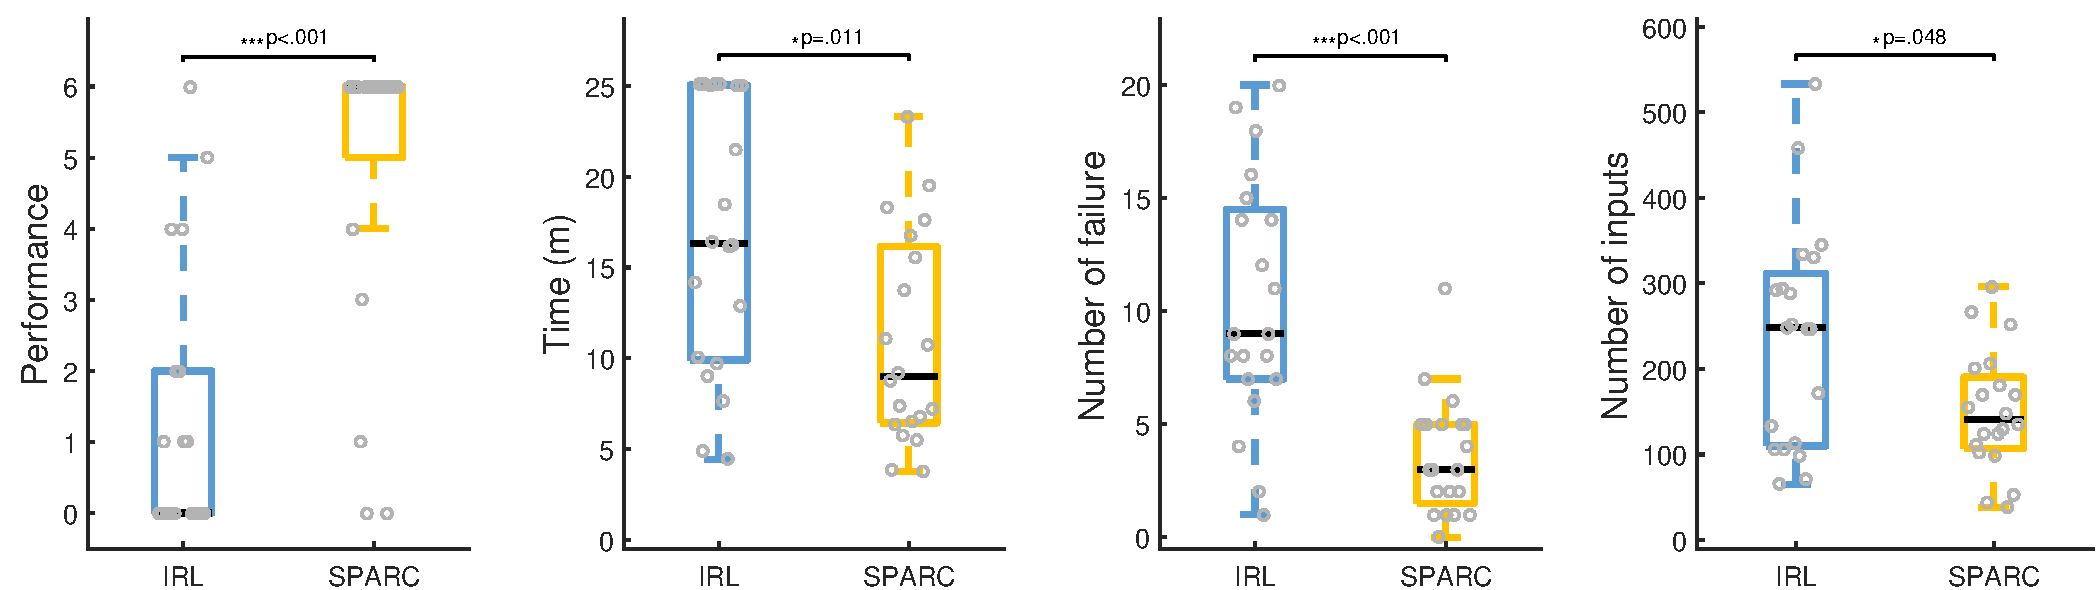
\includegraphics[width=0.9\linewidth]{film.pdf}
    \caption{Comparison of performance, teaching time, number of failure during
    teaching and number of inputs providing for the conditions: IRL and SPARC.}
    \label{fig:film}
\end{figure}

\section{Discussion and Future Work}

These two studies showed that SPARC has promises as interacting principles to
teach a robot how to interact in its environment while not suffering of
classical drawbacks of methods from Reinforcement Learning (poor performance at
the start of the interaction and necessity of large number of samples). However,
these studies were not teaching social behaviours. We are designing a new study
to explore how to teach a robot how to interact with children in an educative
game. 

Children will interact with a touchscreen on a game designed to teach food nets:
which animals eat which ones. And the robot will be used to provide feedbacks
and encouragements to the child. This teaching behaviour will be taught by an
adult using a graphical user interface on a tablet (see Figure~\ref{fig:setup}).

\begin{figure}
    \centering
    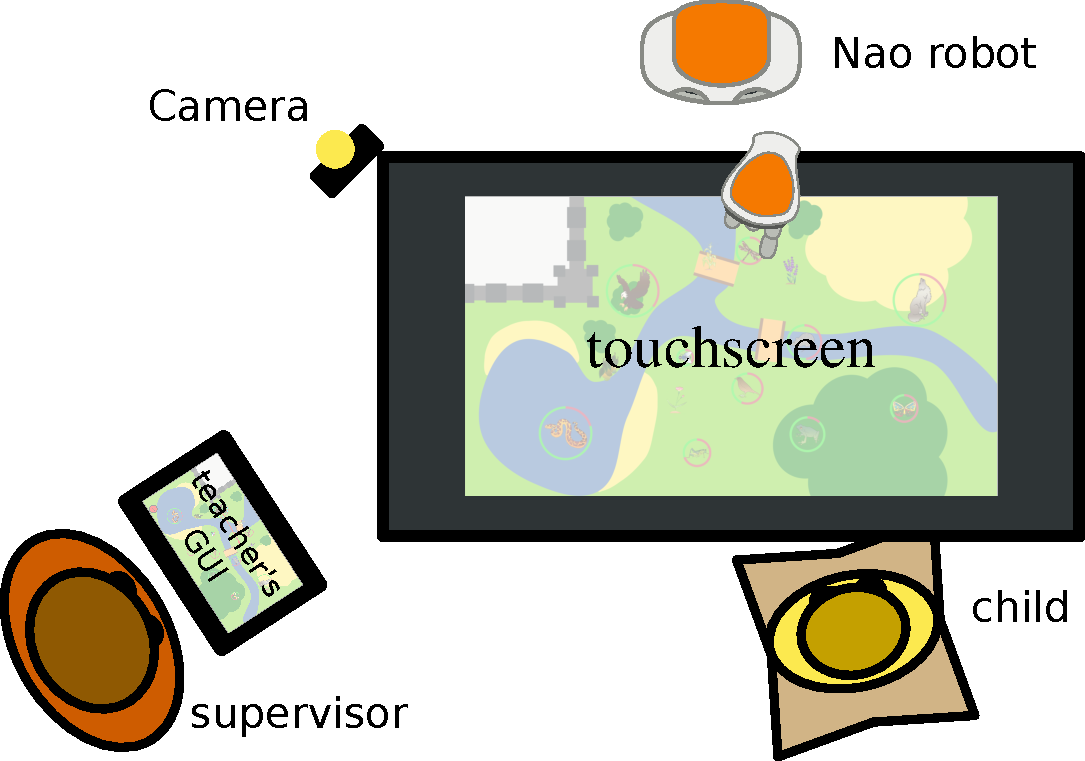
\includegraphics[width=0.9\linewidth]{setup.pdf}
    \caption{Setup for the future study to teach a robot to interact with
    children.}
    \label{fig:setup}
\end{figure}




%\section*{Selected publication}
%\begin{itemize}
%\item E. Senft, P. Baxter, J. Kennedy, and T. Belpaeme, “Sparc:
%            Supervised progressively autonomous robot competencies,” in
%            International Conference on Social Robotics, 2015, pp. 603-612.
%            %\cite{senft2015sparc}
%        \item E. Senft, P. Baxter, J. Kennedy, S. Lemaignan, and T. Belpaeme,
%            “Supevised autonomy for online learning in human-robot interaction,”
%            Pattern Recognition Letters, 2017. %\cite{senft2017supervised}
%\end{itemize}


\bibliographystyle{IEEEtran} \bibliography{biblio}

\end{document}
